\documentclass{article}

\usepackage{graphicx}
\usepackage{tikz}
\usepackage{tikzsymbols}
\usetikzlibrary{calc,patterns,shapes.geometric}
\pagestyle{empty}
\usepackage[margin=0pt]{geometry}
\geometry{papersize={14in,12in}}

\def\centerarc[#1](#2)(#3:#4:#5){\draw[#1] ($(#2)+({#5*cos(#3)},{#5*sin(#3)})$) arc (#3:#4:#5);}

\begin{document}
	\begin{figure}
		\centering
		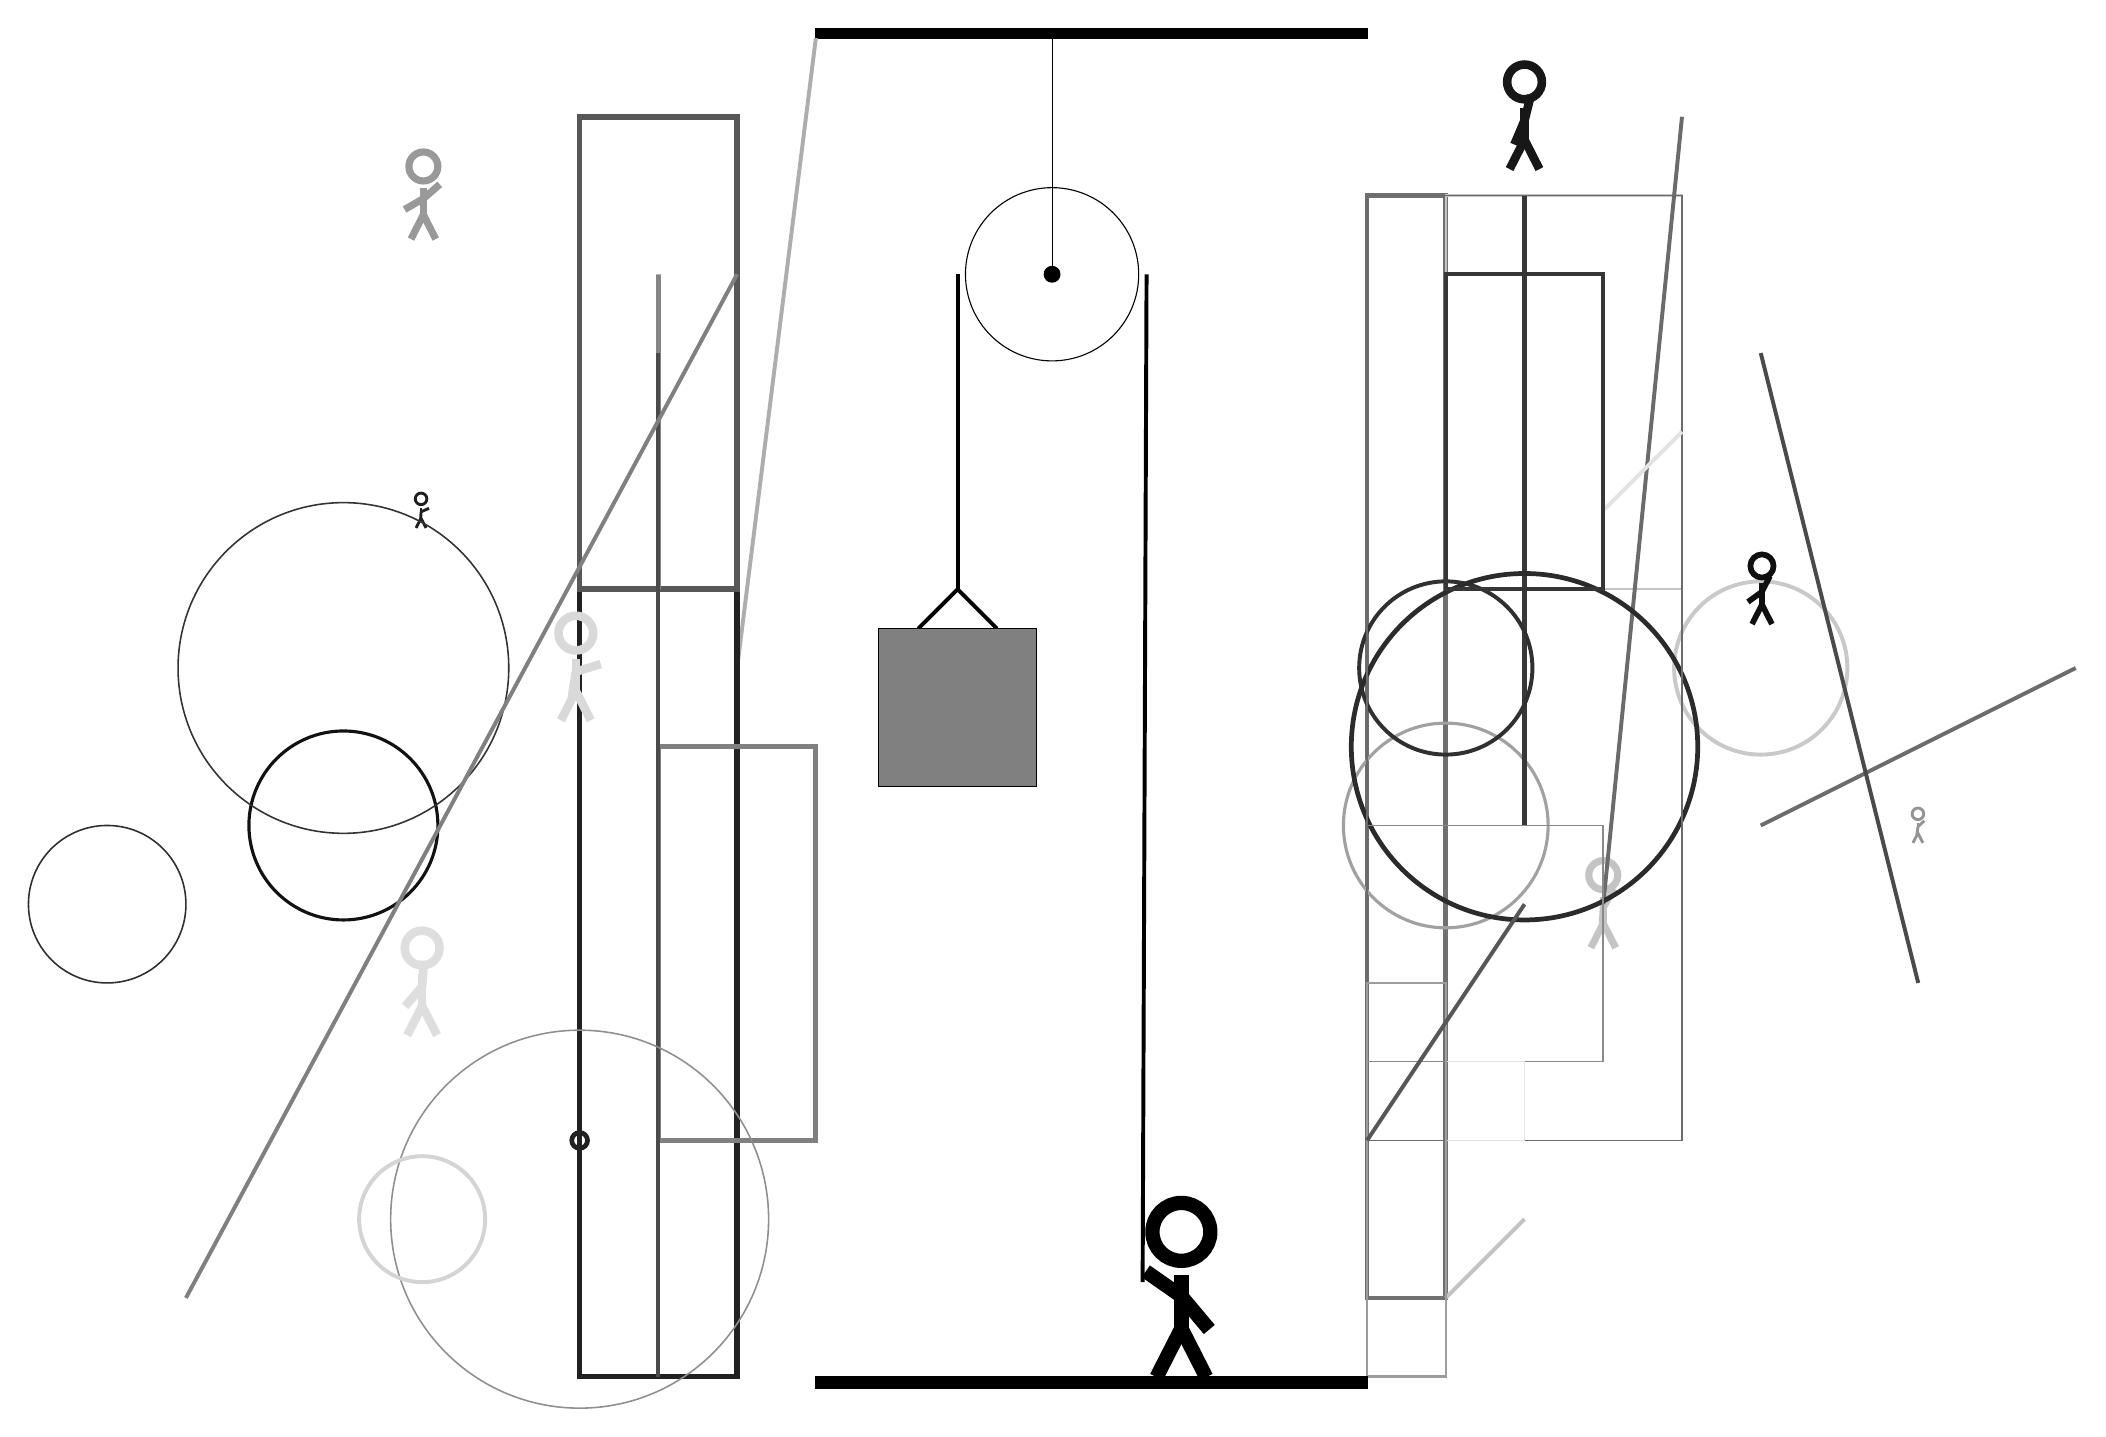
\begin{tikzpicture}
			%%%%% START %%%%%
			
			\draw[fill=black] (-2, 14) rectangle (5, 14.125);
			
			\draw (1, 11) circle (1.1);
			\draw[fill=black] (1, 11) circle (0.1);
			\draw (1, 14) -- (1, 11);
			
			\draw[line width=0.5mm] (-0.7, 6.5) -- (-0.2, 7.0) -- (0.3, 6.5);
			\draw[fill=black!50] (-1.2, 6.5) rectangle (0.8, 4.5);
			
			\draw[line width=0.5mm] (-0.2, 11) -- (-0.2, 7.0);
			\centerarc[line width=0.5mm](1, 11)(0:180:1.2000000000000002);
			\draw[line width=0.5mm](2.2, 11) -- (2.15, -1.8);
			
			\node at (2.6, -1.9) {\Strichmaxerl[10][-35][-50]};
			
			\draw[line width=0.6mm, color=black!56] (6, 12) rectangle (5, -2);
			
			\draw[line width=0.5mm, color=black!32](-3, 6) -- (-2, 14);
			\draw[line width=0.7mm, color=black!87] (-3, -3) rectangle (-5, 7);
			\draw[line width=0.3mm, color=black!23] (6, 7) rectangle (9, 12);
			\node[line width=0.6mm, color=black!13] at (-7, 2) {\Strichmaxerl[6][49][86]};
			\draw[line width=0.7mm, color=black!66] (-3, 7) rectangle (-5, 13);
			
			\node[line width=0.3mm, color=black!40] at (-7, 12) {\Strichmaxerl[5][30][41]};
			
			\draw [line width=0.4mm, color=black!37](6, 4) circle (1.3);
			\node[line width=0.6mm, color=black!88] at (-7, 8) {\Strichmaxerl[2][87][23]};
			
			\draw[line width=0.7mm, color=black!78] (7, 12) rectangle (7, 4);
			
			\draw[line width=0.6mm, color=black!48] (-4, 11) rectangle (-4, 7);
			\draw [line width=0.5mm, color=black!81](6, 6) circle (1.1);
			\draw [line width=0.4mm, color=black!93](-8, 4) circle (1.2);
			
			\node[line width=0.3mm, color=black!23] at (8, 3) {\Strichmaxerl[5][87][60]};
			\draw [line width=0.5mm, color=black!21](10, 6) circle (1.1);
			\draw[line width=0.6mm, color=black!50] (-2, 0) rectangle (-4, 5);
			
			\draw[line width=0.2mm, color=black!47] (-4, 5) rectangle (-4, 8);
			\draw[line width=0.5mm, color=black!58](10, 4) -- (14, 6);
			\node[line width=0.6mm, color=black!42] at (12, 4) {\Strichmaxerl[2][83][43]};
			\draw[line width=0.5mm, color=black!58](8, 3) -- (9, 13);
			\draw[line width=0.5mm, color=black!24](7, -1) -- (6, -2);
			\draw [line width=0.2mm, color=black!80](-8, 6) circle (2.1);
			\draw[line width=0.5mm, color=black!71](-4, 10) -- (-4, -3);
			\draw [line width=0.6mm, color=black!83](7, 5) circle (2.2);
			\draw[line width=0.2mm, color=black!46] (5, 1) rectangle (8, 4);
			
			\draw[line width=0.5mm, color=black!71](10, 10) -- (12, 2);
			
			\draw[line width=0.2mm, color=black!58] (5, 0) rectangle (9, 12);
			\draw[line width=0.5mm, color=black!11](8, 8) -- (9, 9);
			\draw [line width=0.6mm, color=black!87](-5, 0) circle (0.1);
			
			\draw[line width=0.3mm, color=black!39] (6, -3) rectangle (5, 2);
			\draw [line width=0.2mm, color=black!44](-5, -1) circle (2.4);
			
			\node[line width=0.5mm, color=black!94] at (10, 7) {\Strichmaxerl[4][36][63]};
			\draw[line width=0.2mm, color=black!11] (7, 1) rectangle (6, 0);
			
			\node[line width=0.6mm, color=black!15] at (-5, 6) {\Strichmaxerl[6][81][17]};
			\draw[line width=0.3mm, color=black!38] (6, 2) rectangle (6, -3);
			\draw[line width=0.5mm, color=black!50](-3, 11) -- (-10, -2);
			\draw[line width=0.5mm, color=black!79] (6, 7) rectangle (8, 11);
			
			\draw [line width=0.5mm, color=black!17](-7, -1) circle (0.8);
			\node[line width=0.5mm, color=black!91] at (7, 13) {\Strichmaxerl[6][67][76]};
			\draw[line width=0.5mm, color=black!66](7, 3) -- (5, 0);
			
			\draw [line width=0.2mm, color=black!82](-11, 3) circle (1.0);
			
			\draw[fill=black] (-2, -3) rectangle (5, -3.15);
			
			%%%%% END %%%%%
		\end{tikzpicture}
	\end{figure}	
\end{document}